\documentclass[10pt,a4paper,ngerman]{scrartcl}
\usepackage[utf8]{inputenc}
\usepackage[ngerman]{babel}
\usepackage[T1]{fontenc}
\usepackage{amsmath}
\usepackage{amsfonts}
\usepackage{amssymb}
\usepackage{makeidx}
\usepackage{graphicx}
\usepackage{epstopdf}
\usepackage[onehalfspacing]{setspace}
\usepackage{array}
\usepackage{upgreek}
\usepackage{float}
\usepackage{csquotes}
\usepackage{chemformula}
\usepackage{chemgreek}
\usepackage{chemmacros}
\chemsetup{modules=all}
\usepackage{tikz}
\usepackage{siunitx}
\sisetup{locale = DE,per-mode = symbol}
\usepackage{esvect}
\usepackage{geometry}
\usepackage{pdfpages}
\usepackage[font=small]{caption}
%\usepackage[version=4]{mhchem}
\usepackage[backend=biber, style=chem-angew]{biblatex}
\addbibresource{ROMP.bib}
\usepackage{tabularx, booktabs, multirow}
\usepackage[pdfborder={0 0 0}]{hyperref}
\usepackage{scrlayer-scrpage}%Header für die KOMA-script -Klasse
%\usepackage{hyperref}
\usepackage{pgfplots}
\usepackage{textgreek}


\newcommand{\tildenu}{{\fontencoding{LGR}\selectfont\accperispomeni\textnu}}
\captionsetup{format=plain}
\chemsetup[phases]{pos=sub}
\chemsetup[redox]{pos=top}
\chemsetup[redox]{align=center}
%\chemsetup[redox]{explicit-sign=true}
%\chemsetup[redox]{roman=false}
\newcommand{\celsius}{^{\circ}\mathrm{C}}
\parindent0pt
\sloppy
\DeclareChemPhase{\s}{s}
\DeclareChemPhase{\l}{l}
\DeclareChemPhase{\g}{g}
\renewcaptionname{ngerman}{\figurename}{Abb.}
\renewcaptionname{ngerman}{\tablename}{Tab.}
\geometry{bottom=100pt} \geometry{top=80pt}
\newcommand{\m}{\mathrm{m}}
\newcommand{\K}{\mathrm{K}}
\newcommand{\J}{\mathrm{J}}
\newcommand{\gr}{\mathrm{g}}
\newcommand{\kg}{\mathrm{kg}}
\newcommand{\mol}{\mathrm{mol}}
\newcommand{\Pa}{\mathrm{Pa}}
\newcommand{\ad}{\mathrm{ad}}
\newcommand{\de}{\mathrm{de}}
\newcommand{\gmol}{\mathrm{\frac{g}{mol}}}
\newcommand{\JKmol}{\mathrm{\frac{J}{K \cdot mol}}}
\newcommand{\kgmss}{\mathrm{\frac{kg}{m \cdot s^2}}}
\newcommand{\loge}{\mathrm{ln}}


\begin{document}
\begin{titlepage}
	\vspace*{2,5cm}
	\begin{center}
		\begin{LARGE}
			\textbf{Polymer Chemie}\\
			\textbf{Ring opening Methathesis Polymerization (ROMP)}\\
		\end{LARGE}
		\vspace{1cm}
		\textbf{Universität Stuttgart}\\
		\vspace*{1,5cm}
		\begin{tabular}{lp{7,5cm}l}
			Author 1:     &Laurens Viehoff\\
            Author 2:     &Felix Roth\\   
			E-Mail 1:      &st183688@stud.uni-stuttgart.de\\
            E-Mail 2:      &st188157@stud.uni-stuttgart.de  \\
			Student-ID 1: & 3676761   \\ 
            Student-ID 2: & 3711192 \\ \\
			Assistentin:  &   \\ \\ 
		\end{tabular}
	\end{center}

    
\end{titlepage}
\thispagestyle{empty}
\renewcommand{\thepage}{\arabic{page}}
\newpage
\tableofcontents
\setcounter{page}{1}
\renewcommand{\thepage}{\arabic{page}}
\newpage


\section{Theorie}

	\subsection{Metallische Polyinsertionen}

		Eine der Bekanntesten Polyinsertionen ist dioe Ziegler-Natta-Reaktion.
		Dabei werden Katalysatoren verwendewt welche ein Element der Gruppen 1-3 mit einem Übergangsmetall der 4-8 Gruppe gebunden haben.
		Beispiele hierfür wären zB. Metallhydride oder Arylidenverbindungen. 
		Im falle der Ziegler-Natta ist besteht der Katalysator aus \ch{TiCl4} mit \ch{Et3Al}.
		Die Metallische Polyinsertionen lassen sich in eine Monometallische und eine Bimetallische Polymerisation unterteilen.
		Beide machen sich jedoch die koordinationseigenschaften des Übergangsmetalls zu nutze.
		So koordiniert eine Doppelbindung an einen Freie stelle des Metalls. 
		Dabei bildet sich mit einem Rest an einer anliegenden Stelle ein viergliedriger übergangszustand.
		Anschließend klappen die bindungen so um, dass der rest an die eine seite der Doppelbindung übertragen wird.
		Die Kette ist somit um den Rest des Olefins gewachsen.

			\begin{figure}[H]
				\centering
				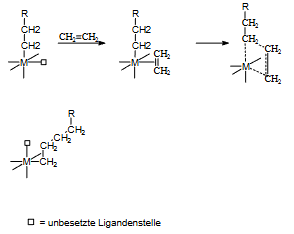
\includegraphics[scale = 0.75]{Bilder/Monometall.png}
				\caption{}
				\label{Monometall}
			\end{figure}

		Wichtig hierbei ist, dass der Metallkomplex nicht an der Wachstumsreaktion beteiligt ist und lediglich
		das neue Monomer an das Polymer koordiniert.\\
		Die Reaktion kann auf drei unterschiedliche weisen abgebrochen werden.
		So kann die Reaktion durch eine $\beta$-H-Eliminierung abgebrochen werden.
		Oder durch eine Übertragung auf das Monomer, und letzteres besteht die Möglichkeit einer Molekulargewichtsregelung durch \ch{H2}.\\

		Beim Bimetallischen hingegen sind wie der Name bereits sagt zwei Metallatome beteiligt.
		Dabei wechselwirken die $\pi$-Elektronen des Olefins mit den Orbitalen des Übergangsmetalls.
		Wichtig ist dabei, dass selbst nach der koordination des Olefins an das Metall, keine freihe drehbarkeit zwischen C-C möglich ist.
		Genauso beeinträchtigt bleibt die freihe drehbarkeit zwischen Metall-Kohlenstoff-Bindung.
		Dies spielt eine große Rolle, da dadurch der Rest welcher am Olefin gebunden ist seine relative Position inrichtung der Methylgruppe behält.
		Anschließend bildet sich ein Ring wodurch der Elektronenüberlapp eine neue $\sigma$-Bindung zwischen C(1) und C(3) gebildet wird. 
		Dabei wird die Al-C(3)-Bindung gekappt und es kann sich der Ausgangskomplex mit dem neu hinzugefügten Rest bilden.

			\begin{figure}[H]
				\centering
				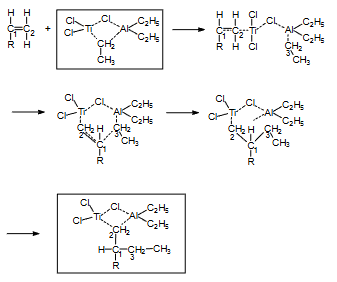
\includegraphics[scale = 0.75]{Bilder/Bimetallisch.png}
				\caption{}
				\label{}
			\end{figure}
		
		Meist wird bei der verwendung dieser Mechanismen Monomere wie Propen oder Styrol verwendet,
		durch welche unterschiedliche stereoreguläre Polymerketten gebildet werden können.
		Dabei wird zwischen isotaktisch (in Abb. \ref{taktizitäen} mitte), syndiotaktisch (in Abb. \ref{taktizität} rechts) und in ataktisch (in Abb. \ref{taktizität} links) unterschieden.
		Bei ersterem zeigen die Reste immer in die selbe Richtung es etsteht die Konfiguration RRRRR. 
		Bei der syndiotaktischen hingegen sind diese alternierend, es ergibt sich die konfiguration RSRSRS. 
		Bei letzeren ist die abfolge komplett zufällig.
		Diese Taktizität hat einen großen Einfluss auf die Eigenschaften des Polymers.
		
			\begin{figure}[H]
				\centering
				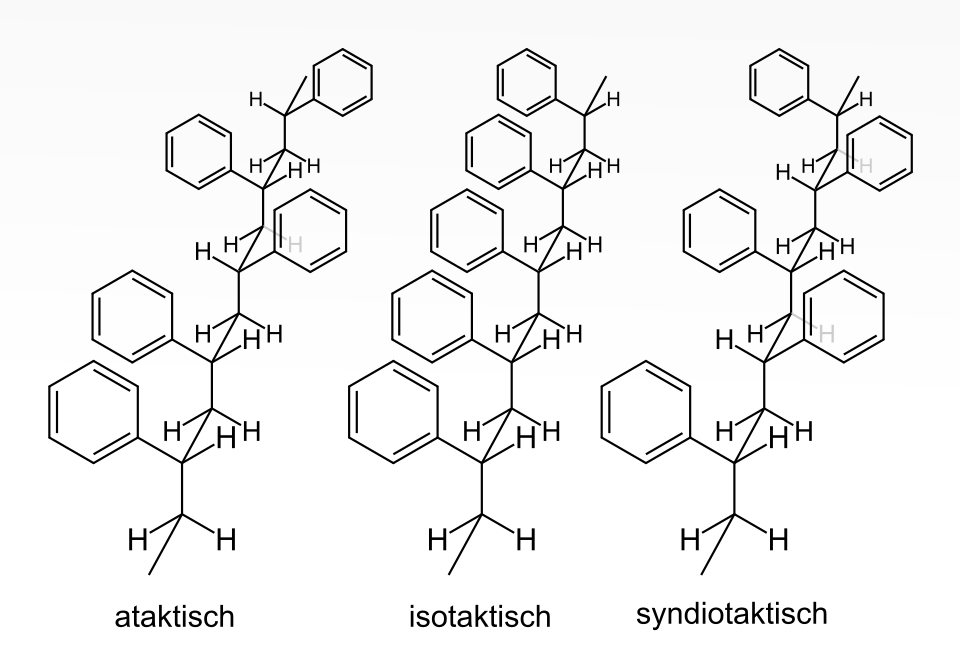
\includegraphics[scale = 0.25]{Bilder/taktizität.png}
				\caption{}
				\label{taktizität}
			\end{figure}
		
		
	\subsection{Ring öffnende Methathespolymerisation}

		Die Ring öffnende Methathesenpolymerisation (ROMP) läuft im allgemeinen nach dem Mechanismus der Olefinmethathese.
		Bei diesem findet ein Austausch von Alkenylgruppen zweier Olefine statt. 
		Dies läuft in Gegenwart eines Organo-Metallischen-Katalysators.
		Einige wichtige Namen dieser Katalysechemie sind Grubbs und Schrock.
		Im allgemeinen reagieren die beiden Olefine in einer [2+2] Zykloaddition.
		Das dadurch entstandene Metallcyclobutan-Intermediat kann wiederum in einer [2+2] Zykloreversion das Produkt bilden.
		Das Metall wird dabei selbst als Metallalkyliden abgespalten.
		Der große vorteil diesert Reaktionen ist, dass jeder schritt im großen und ganzen reversibel ist.
		Ein nachteil welcher diese Irreversibelität mit sich bringt ist, dass eine große kontrolle über die Triebkraft notwendig sein muss.

			\begin{figure}[H]
				\centering
				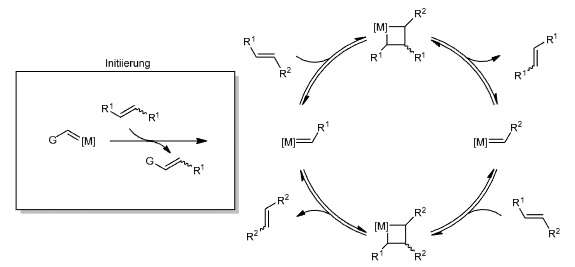
\includegraphics[scale = 0.75]{Bilder/Methathesezyklus.png}
				\caption{}
				\label{Methathesezyklus}
			\end{figure}

		In unserem Fall wird der Grubbs-Katalysator der ersten Generation verwendet welcher auch in Abb. \ref{Grubbs} zu sehen ist.
		Im allgemeinen ist es wichtig zu wissen, dass es viele unterschiedliche Katalysatoren für unterschiedliche gebiete mit unterschiedlichem Nutzen gibt.
		
			\begin{figure}[H]
				\centering
				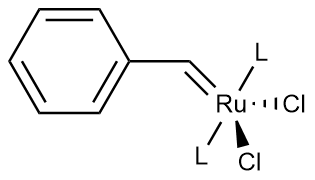
\includegraphics[scale = 0.5]{Bilder/Grubbs.png}
				\caption{}
				\label{Grubbs}
			\end{figure}

		Im falle der ROMP wird diese Methathese mittels eines monozyklischen Olefins durchgeführt welcher im laufe des Kettenwachstums geöffnet wird.
		Die wie bereits oben genannte Triebkrafft liegt hierbei in der Ringspannung welche durch das üffnen verloren geht.
		Der allgemeine Ablauf der ROMP ist in Abb. \ref{ROMP} gezeigt.

			\begin{figure}[H]
				\centering
				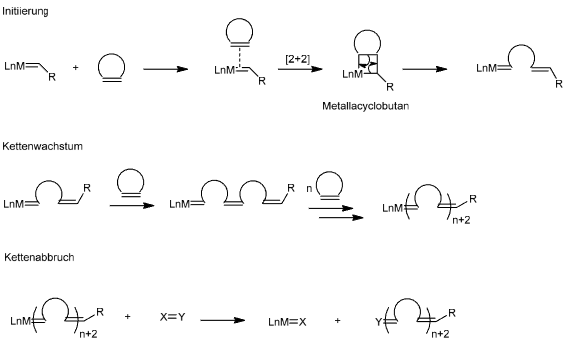
\includegraphics[scale = 0.75]{Bilder/ROMP.png}
				\caption{}
				\label{ROMP}
			\end{figure}

\section{Durchführung}

	In allen versuchsteilen sollte unter schlenk Bedingungen gearbeitet werden.
	Jedoch wurde im ersten Versuchsteil nach absprache mit dem Assistenten nicht unter schlenk gearbeitet, 
	da dies ausprobiert werden sollte da es theoretisch keinen unterschied machen sollte.

	\subsection{Polyinsertion}

		In einem Kolben mit Septum wurde Heptan (\SI{25}{ml} aus der SPS) vorgelegt.
		Es wurde eine Spritze mit \SI{0.5}{ml} \ch{TiCl4} zugegeben. Anschließend sollten \SI{12.5}{ml} einer Aluminiumalkyl Lösung im zeitraum von 20 min zugegeben werden.
		Dieser Schritt wurde jedoch falsch gemacht und es wurde alles schnell zugegen.
		Der Kolben wurde während des zugebens mit einem Wasserbad gekühlt.
		Nach 10 min wurden \SI{12.5}{ml} Styrol auf einmal zugegeben und bei 74°C für 3-4h geheitzt.
		Anschließend wird auf Raumtemperatur abgekühlt und die Reaktion wird mit \SI{100}{ml} in Methanol gelöster \ch{HCl} abgebrochen.
		Das Polymer wurde in Methanol gefällt und abfiltriert und gewaschen.
		Das Produkt wurde im Vakuumtrockenschrank bei 60°C getrocknet.
		
	\subsection{ROMP}

		In einem Schlenkkolben wurden \SI{20}{ml} trockenes DCM vorgelegt. 
		Es wurde \SI{1.00}{g}(\SI{3,29}{mmol}) Monomer eingewogen un in den Kolgen gegeben.
		Der Katalysator (\SI{43}{mg}, 1mol\%) wurden in ein Schnappdeckelglas eingewogen und in \SI{2}{ml} trockenem
		DCM gelöst.
		Die Lösung wurde anschließend in einem Schuss zugegeben und die Lösung wurde für 1 Stunde bei Raumtemperatur gerührt.
		Nach einer Stunde wurde eine Spritze (\SI{2}{ml}) entnommen und in Methanol gegeben.
		Zur restlichen Lösung wurden \SI{20}{ml} Ethylvinylether zugegeben und weitere 10 Minuten gerührt.
		Anschließend wird auch hier das Polymer in Methanol gefällt abfiltriert und getrocknet.

\section{Auswertung}

	

\section{Fragen}

	\subsection{Polyinsertion}

		\subsubsection{Frage 1}

			Die Extraktion mit Methylethylketon und Toluol sorgt für eine Auftrennung des Produkts, welches möglicherweise aus Polymer und davon eingeschlossenem Titan- 
			und Aluminiumalkylen besteht. Somit wird im Ganzen das Polymer sauberer.

		\subsubsection{Frage 2}

			Verwendet wurden bei der Reaktion \SI{0,5}{ml} $\ch{TiCl4}$ und \SI{12,5}{ml} Styrol. Mit den entsprechenden Dichten und molaren Massen, entspricht das einem 
			Verhältnis von 

			\begin{equation}
				\frac{n_\text{Ti}}{n_\text{Styrol}} = \frac{\frac{\rho_\text{Ti} \cdot V_\text{Ti}}{M_\text{Ti}}}{\frac{\rho_\text{Styrol} \cdot V_\text{Styrol}}{M_\text{Styrol}}} = \frac{\frac{\SI{1,728}{\frac{g}{ml}} \cdot \SI{0,5}{ml}}{\SI{189,71}{\frac{g}{mol}}}}{\frac{{\SI{0,91}{\frac{g}{ml}} \cdot \SI{12,5}{ml}}}{\SI{104,15}{\frac{g}{mol}}}} = 0,0417 \text{.}
			\end{equation}

			Die Stoffmengenkonzentration des Katalysators entspricht dabei der Stoffmengenkonzentration des $\ch{TiCl4}$ für das ganze Volumen und somit

			\begin{equation*}
				M_\text{\ch{TiCl4}} = \frac{\frac{\rho_\text{Ti} \cdot V_\text{Ti}}{M_\text{Ti}}}{V_\text{ges}} = \frac{\frac{\SI{1,728}{\frac{g}{ml}} \cdot \SI{0,5}{ml}}{\SI{189,71}{\frac{g}{mol}}}}{\SI{25}{ml} + \SI{0,5}{ml} + \SI{12,5}{ml} + \SI{12,5}{ml}} = \SI{90,185}{\frac{mmol}{l}} \text{.}
			\end{equation*}

		\subsubsection{Frage 3}

			Die nachfolgende Abbildung zeigt die Fischer- und die Natta-Projektion auf.

			\begin{figure}[H]
				\centering
				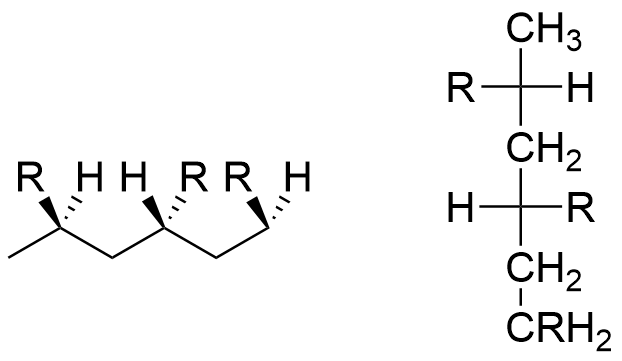
\includegraphics[scale = 0.4]{Bilder/Natte-Fischer-Projektion.png}
				\caption{Abgebildet ist links die Natta- und rechts die Fischer-Projektion des selben hypothetischen Oligomeren.}
				\label{NattaFischerProjektionabb}
			\end{figure}

			Bei der Natta-Prjektion wird die Orientierunge der Substituenten durch Keile oder Striche gekennzeichnet, während bei der Fischer Projektion die fortführende 
			Kette immer nach oben und unten geschrieben wird und die Substituenten rechts und links abgehen. Dabei wird auf das Substitutionstetraeder so draufgeschaut, dass 
			die fortführende Kette nach hinten zeigt und vorne die Substituenten stehen. Nach links zeigen dann die Substituenten, welche in der Natta-Projektion nach vorne 
			stehen und umgekehrt.

		\subsubsection{Frage 5}

			Bei LDPE und HDPE ist die Dichte der Hauptunterschied, was dadurch Zustande kommt, dass die Polymerketten bei LDPE nur amorphe Strukturen bilden und HDPE 
			teilkristallin ist. 


		\subsubsection{Frage 6}

			Durch den Sauerstoff in der Etherbindung, würde dieser im bimetallischen Mechanismus zum Titan koordinieren und diesen so desaktivieren.

		\subsubsection{Frage 7}

			HDPE besteht aus teilkristallinen Strukturen aus linearem Polyethylen. Bei LDPE ist die Struktur amorph, da die Ketten zusätzlich verzweigt sind. LLDPE ist 
			ebenfalls amorph, allerdings sind die Verzwigungen weniger lang als bei LDPE, wodurch die Dichte etwas ansteigt. Diese und weitere Strukturen sind nochmal in 
			Abbildung \ref{ROMPstrukturen} aufgeführt.

			\begin{figure}[H]
				\centering
				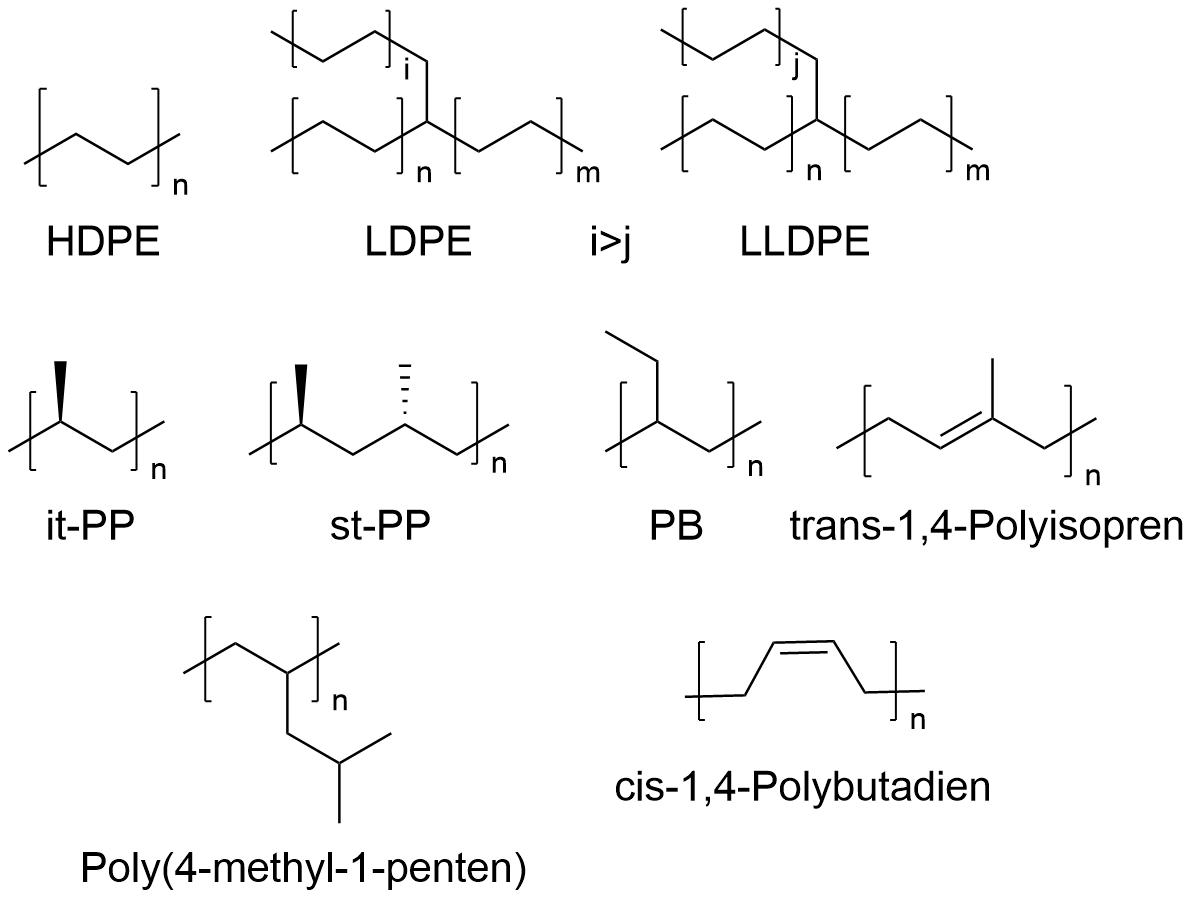
\includegraphics[scale = 0.4]{Bilder/StrukturenROMP.png}
				\caption{Abgebildet sind die Strukturen der Polymere.}
				\label{ROMPstrukturen}
			\end{figure}


	\subsection{ROMP}

		\subsubsection{Frage 1}

			Beim ersten Fällen, bildete sich ein roter Polymerklumpen, der beim zweiten Fällen nicht beobachtet wurde. Das liegt daran, dass beim ersten Fällen noch der 
			Grubbs-Katalysator die Endgruppe bildete und beim zweiten Fällen zuvor entfernt wurde.

		\subsubsection{Frage 2}

			Ethylvinylether bricht die Reaktion ab und ersetzt die Endgruppe. Dabei wird nämlich der Ruthenium-Kat gegen ein Kohlenstoff substituiert. Die Reaktion ist 
			anschließend aufgeführt. 

			\begin{figure}[H]
				\centering
				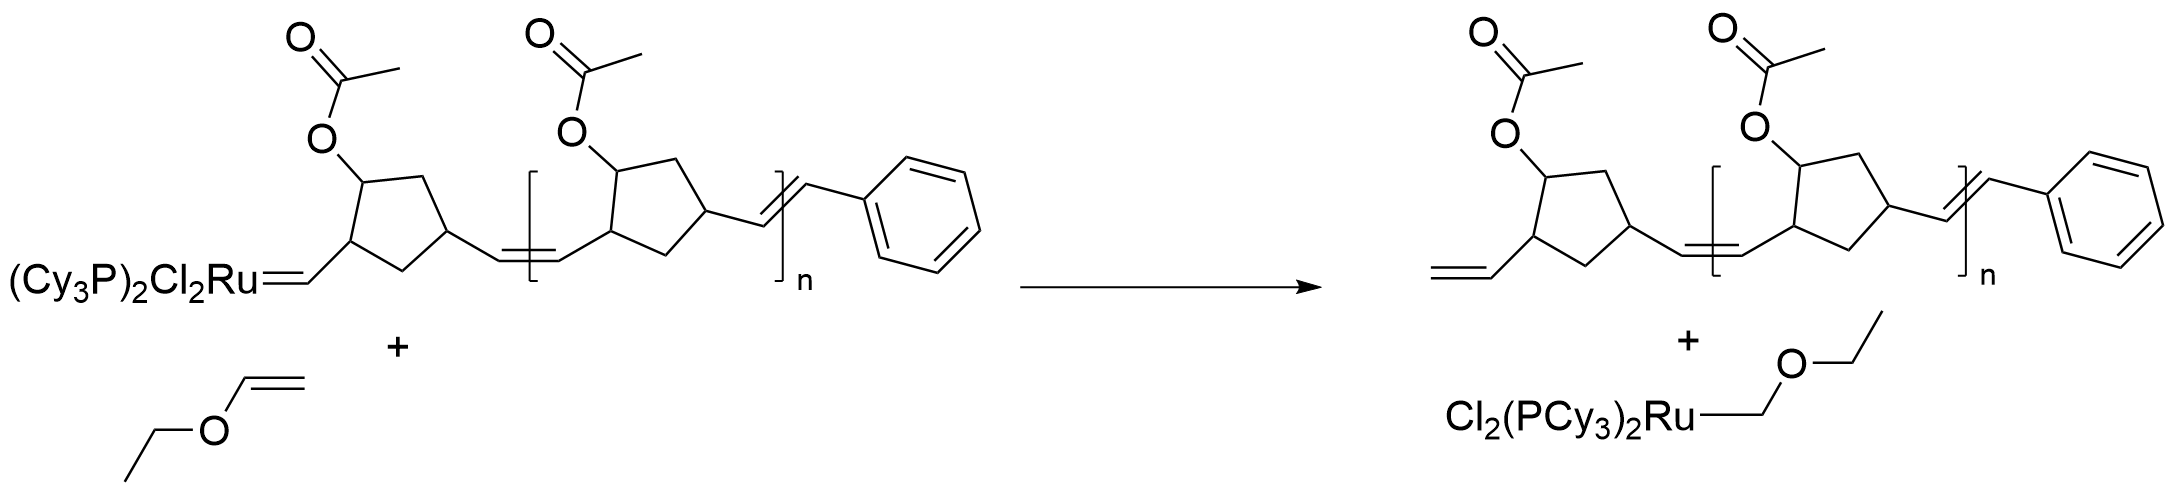
\includegraphics[scale = 0.4]{Bilder/ROMPabbruchethylvinylether.png}
				\caption{Reaktionsgleichung des Abbruchreaktion zwischen dem Grubbs-Polymer und Ethylvinylether.}
				\label{ROMPethylvinyletherabbruch}
			\end{figure}

			Der Grund für die Wahl von Ethylvinylether ist die definierte Endgruppe. Denn bei der Koordinierung von Ethylvinylether an Ruthenium, koordiniert dieses immer 
			nach der Weise aus Reaktion \ref{ROMPethylvinyletherabbruch}. Mit 1-Penten wäre die Endgruppe nicht bekannt und wäre statistisch Verteilt.

		\subsubsection{Frage 3}

			Der Katalysator muss bei der Reaktion so schnell wie möglich hinzugegeben werden, um die Polydispersität möglichst eng zu halten und alle Polymere gleichzeitig 
			starten zu lassen.

		\subsubsection{Frage 4}

			Das theoretische Molekulargewicht wird über die Monomermasse und die Katalysatorstoffmenge bestimmt. Damit ergibt sich eine molekulare Masse von

			\begin{equation*}
				M_\text{theo} = \frac{m_\text{Mono}}{n_\text{kat}} = \frac{\SI{1}{g}}{\SI{0,0329}{mmol}} = \SI{30395,14}{\frac{g}{mol}} \text{.}
			\end{equation*}



		\subsubsection{Frage 5}

			Den Katalysator kann nach der desaktivierung mit Ethylvinylether nicht erneut verwendet werden, da der Rest zu inreaktiv ist. Allerdings kann der Katalysator 
			chemisch regeneriert werden, indem der Rest substituiert wird. 

		\subsubsection{Frage 6}

			Um das Polymer löslicher zu gestallten, müssen die Seitenketten variiert werden. Mit Phenylresten wären das Polymer möglich in Toluol zu lösen, mit ionischen 
			Seitenketten wäre es möglich es in Wasser zu lösen. Die Faktoren die eine Rolle spielen sind Polarität und Bildung guter zwischermolekularer Wechselwirkungen.

		\subsubsection{Frage 7}

			Die Wahl des Katalysators kann die Reaktionsgeschwindigkeit verändern. Bei der koordinierung der Monomere an den Ruthenium-Kern muss dieser einen Substituenten 
			abspalten um das Monomer zu koordinieren. Die Wahl dieses Substituenten ist dabei dann Geschwindigkeitsbestimmend. Ist die Dativbindung zwischen dem Liganden und 
			dem Ruthenium-Kern beispielsweise stärker, ist die Reaktion verlangsamt. Ist aber die Bindung schwächer, ist die Reaktion schneller.
		
		\subsubsection{Frage 8}

			Der Ausgangskatalysator besitzt ein Carben, welches im singulett oder triplett Zustand vorliegen kann. Je nach dem wäre dieses Signal hochfeld verschoben. Der 
			weiteren ist die propagierede Spezies ein Cyclobutanderivat, bei welchem nur einfach Bindungen vorliegen und die chemische Umgebung unterschiedlich ist. 
			Dementsprechend wäre dieses Signal wieder Verschoben und von dem Signal des Ausgangskatalysators verschieden.

		\subsubsection{Frage 9}

		

\printbibliography

\end{document}